\makeatletter
\def\input@path{{../projektdokumentation/}}
\makeatother

% Dokumentklassen sættes til memoir.
% Manual: http://ctan.org/tex-archive/macros/latex/contrib/memoir/memman.pdf
\documentclass[a4paper,11pt,twoside,openright,article]{memoir}
\setlrmarginsandblock{*}{2.5cm}{0.75} % højre og venstre 
\setulmarginsandblock{3cm}{*}{1.2} % top og bund 
\checkandfixthelayout[nearest] % specifikt valg af højde algoritme
 
% Danske udtryk (fx figur og tabel) samt dansk orddeling og fonte med
% danske tegn. Hvis LaTeX brokker sig over æ, ø og å skal du udskifte
% "utf8" med "latin1" eller "applemac". 
\usepackage[utf8]{inputenc}
\usepackage[danish]{babel}
\usepackage[T1]{fontenc}
\usepackage{mflogo}

%sexy pdf'er
%\usepackage[export]{adjustbox}
\usepackage{pdfpages}
\usepackage{pdflscape}

%Kompakte lister
\usepackage{paralist}
 
% Matematisk udtryk, fede symboler, theoremer og fancy ting (fx kædebrøker)
\usepackage{amsmath,amssymb}
\usepackage{bm}
\usepackage{amsthm}
\usepackage{mathtools}
\parindent=0pt 

% Fancy ting med enheder og datatabeller. Læs manualen til pakken
% Manual: http://www.ctan.org/tex-archive/macros/latex/contrib/siunitx/siunitx.pdf
\usepackage{siunitx}
 
%Fancy headers, 
%Manual: https://www.sharelatex.com/learn/Headers_and_footers
\let\footruleskip\undefined
\usepackage{fancyhdr}
\pagestyle{fancy}

 
% Indsættelse af grafik. og man kan rotere tekst in line
\usepackage{graphicx} 
\usepackage{fix-cm} 
\usepackage{soul}
\sodef\an{}{0.13em}{0em}{0em} \sodef\ann{}{0.13em}{0.5em}{0em}
 
%Fancy tabeller.
%\usepackage[table]{xcolor}
\usepackage{multirow}
\usepackage{rotating} %sidewaystables!
\usepackage{longtable} %tables spanning multible pages.
\usepackage{tablefootnote} %for at indstætte fornoter i tabeller.
\usepackage{hhline} %Fixer farvede felter
\usepackage{ltxtable} %Longtabular X
\usepackage{tabularx} %Med dynamisk bredte

%URL fodnoter
\usepackage{url}

% Reaktionsskemaer. Læs manualen for at se eksempler.
% Manual: http://www.ctan.org/tex-archive/macros/latex/contrib/mhchem/mhchem.pdf
\usepackage[version=3]{mhchem}

%Lav chapter clickable og fjern border
\usepackage{hyperref}
\hypersetup{
    colorlinks,
    citecolor=black,
    filecolor=black,
    linkcolor=black,
    urlcolor=black
}

%Table of contents settings
\setsecnumdepth{subsection} % organisational level that receives a numbers
\settocdepth{subsection}   % print table of  for level 3

%Til programkode
\usepackage{listings}
\usepackage{color}

\definecolor{dkgreen}{rgb}{0,0.6,0}
\definecolor{gray}{rgb}{0.5,0.5,0.5}
\definecolor{mauve}{rgb}{0.58,0,0.82}
 
\lstset{ 
  language=C++,                % the language of the code
  basicstyle=\footnotesize,           % the size of the fonts that are used for the code
  numbers=left,                   % where to put the line-numbers
  numberstyle=\tiny\color{gray},  % the style that is used for the line-numbers
  stepnumber=1,                   % the step between two line-numbers. If it's 1, each line 
                                  % will be numbered
  numbersep=5pt,                  % how far the line-numbers are from the code
  backgroundcolor=\color{white},      % choose the background color. You must add \usepackage{color}
  showspaces=false,               % show spaces adding particular underscores
  showstringspaces=false,         % underline spaces within strings
  showtabs=false,                 % show tabs within strings adding particular underscores
  frame=single,                   % adds a frame around the code
  rulecolor=\color{black},        % if not set, the frame-color may be changed on line-breaks within not-black text (e.g. commens (green here))
  tabsize=2,                      % sets default tabsize to 2 spaces
  captionpos=b,                   % sets the caption-position to bottom
  breaklines=true,                % sets automatic line breaking
  breakatwhitespace=false,        % sets if automatic breaks should only happen at whitespace
  title=\lstname,                   % show the filename of files included with \lstinputlisting;
                                  % also try caption instead of title
  keywordstyle=\color{blue},          % keyword style
  commentstyle=\color{dkgreen},       % comment style
  stringstyle=\color{mauve},         % string literal style
  escapeinside={\%*}{*)},            % if you want to add LaTeX within your code
  morekeywords={*,...},               % if you want to add more keywords to the set
  rangeprefix=//----------,			%Used for sexy code includes
  rangesuffix=----------,			%---||---
  includerangemarker=false,			%---||---
  literate=
  {á}{{\'a}}1 {é}{{\'e}}1 {í}{{\'i}}1 {ó}{{\'o}}1 {ú}{{\'u}}1
  {Á}{{\'A}}1 {É}{{\'E}}1 {Í}{{\'I}}1 {Ó}{{\'O}}1 {Ú}{{\'U}}1
  {à}{{\`a}}1 {è}{{\`e}}1 {ì}{{\`i}}1 {ò}{{\`o}}1 {ù}{{\`u}}1
  {À}{{\`A}}1 {È}{{\'E}}1 {Ì}{{\`I}}1 {Ò}{{\`O}}1 {Ù}{{\`U}}1
  {ä}{{\"a}}1 {ë}{{\"e}}1 {ï}{{\"i}}1 {ö}{{\"o}}1 {ü}{{\"u}}1
  {Ä}{{\"A}}1 {Ë}{{\"E}}1 {Ï}{{\"I}}1 {Ö}{{\"O}}1 {Ü}{{\"U}}1
  {â}{{\^a}}1 {ê}{{\^e}}1 {î}{{\^i}}1 {ô}{{\^o}}1 {û}{{\^u}}1
  {Â}{{\^A}}1 {Ê}{{\^E}}1 {Î}{{\^I}}1 {Ô}{{\^O}}1 {Û}{{\^U}}1
  {œ}{{\oe}}1 {Œ}{{\OE}}1 {æ}{{\ae}}1 {Æ}{{\AE}}1 {ß}{{\ss}}1
  {ç}{{\c c}}1 {Ç}{{\c C}}1 {ø}{{\o}}1 {å}{{\r a}}1 {Å}{{\r A}}1
  {€}{{\EUR}}1 {£}{{\pounds}}1
}

%Til at udregne forskel mellem sider, brug \pagedifference{A}{B} mellem to labels A og B.
\usepackage{refcount}
\newcommand{\pagedifference}[2]{%
  \number\numexpr\getpagerefnumber{#2}-\getpagerefnumber{#1}\relax}
 
%Til at lave referencer med:
\usepackage{cite}

%Til at lave eksterne \ref til \labels
\usepackage{xr}

%Til at lave \Beam (DC symbol)
\usepackage{marvosym}

%Forsøg på nice lister i tabeller
\usepackage[shortlabels]{enumitem}

\newenvironment{packed_enum}{
\begin{enumerate}[1., topsep=0pt, nosep, partopsep=0pt, itemsep=0pt, parsep=0pt]
}{\end{enumerate}}

\newenvironment{packed_item}{
\begin{itemize}[•, topsep=0pt, nosep, partopsep=0pt, itemsep=0pt, parsep=0pt]
}{\end{itemize}}

%Lækker kommando til at skrive I2C flot uden at bruge \textsuperscript hver gang:
\newcommand*{\IIC}{\texorpdfstring{I\textsuperscript{2}C }{I2C }}

%Lorem ipsum
\usepackage{lipsum}


\usepackage{longtable}
\usepackage{array} % for extrarowheight

%Juicy columntypes - http://tex.stackexchange.com/questions/12703/how-to-create-fixed-width-table-columns-with-text-raggedright-centered-raggedlef
\newcolumntype{L}[1]{>{\raggedright\let\newline\\\arraybackslash\hspace{0pt}}p{#1}}
\newcolumntype{C}[1]{>{\centering\let\newline\\\arraybackslash\hspace{0pt}}p{#1}}
\newcolumntype{R}[1]{>{\raggedleft\let\newline\\\arraybackslash\hspace{0pt}}p{#1}}
\newcolumntype{Z}{>{\raggedright\arraybackslash}X}

%Dejlig kommando til at få nye kapitler på højre side
\newcommand*\cleartorightpage{%
	\clearpage
 	\checkoddpage
	\ifoddpage
  		%do nothing
	\else
		\thispagestyle{empty}
		\mbox{}
 		\clearpage
	\fi
}


%Hacky løsning til at ordne indholdsfortegnelsen.. Why memoir class.. WHY??!
\renewcommand*{\cftdotsep}{1}
\setpnumwidth{3em}
\setrmarg{4em}

%Bugfix til Longtables
\makeatletter
\def\LT@start{%
  \let\LT@start\endgraf
  \endgraf\penalty\z@\vskip\LTpre
  \dimen@\pagetotal
  \advance\dimen@ \ht\ifvoid\LT@firsthead\LT@head\else\LT@firsthead\fi
  \advance\dimen@ \dp\ifvoid\LT@firsthead\LT@head\else\LT@firsthead\fi
  \advance\dimen@ \ht\LT@foot
  \edef\restore@vbadness{\vbadness\the\vbadness\relax}% (added)
  \vbadness=\@M % (added)
  \dimen@ii\vfuzz
  \vfuzz\maxdimen
    \setbox\tw@\copy\z@
    \setbox\tw@\vsplit\tw@ to \ht\@arstrutbox
    \setbox\tw@\vbox{\unvbox\tw@}%
  \vfuzz\dimen@ii
  \restore@vbadness % (added)
  \advance\dimen@ \ht
        \ifdim\ht\@arstrutbox>\ht\tw@\@arstrutbox\else\tw@\fi
  \advance\dimen@\dp
        \ifdim\dp\@arstrutbox>\dp\tw@\@arstrutbox\else\tw@\fi
  \advance\dimen@ -\pagegoal
  \ifdim \dimen@>\z@\vfil\break\fi
      \global\@colroom\@colht
  \ifvoid\LT@foot\else
    \advance\vsize-\ht\LT@foot
    \global\advance\@colroom-\ht\LT@foot
    \dimen@\pagegoal\advance\dimen@-\ht\LT@foot\pagegoal\dimen@
    \maxdepth\z@
  \fi
  \ifvoid\LT@firsthead\copy\LT@head\else\box\LT@firsthead\fi\nobreak
  \output{\LT@output}%
}
\makeatother

%Debugging
%\overfullrule=2cm

\title{Projektdokumentation \\ AU2 \\ Gruppe 1}
\author{4. Semesterprojekt E4PRJ4 \\ Ingeniørhøjskolen, Aarhus Universitet\\ Vejleder: Arne Justesen}
\date{\today}

\begin{document}
\fancyhf{} %Clear all header/footers
\frontmatter
\maketitle
\vfill

\begin{table} [h]
	\centering
	\begin{tabular}{|l|r|l|}
	\hline 
	\textbf{Navn} & \textbf{Studienummer} & \textbf{Underskrift~~~~~~~~~~~~~~~~~~~~} \\ \hline
	Kristian Thomsen & 201311478 & \\ && \\ \hline
	Philip Krogh-Pedersen & 201311473 & \\ && \\ \hline
	Lasse Barner Sivertsen & 201371048 & \\ && \\ \hline
	Henrik Bagger Jensen & 201304157 & \\ && \\ \hline
	Kenn Hedegaard Eskildsen & 201370904 & \\ && \\ \hline
	Karsten Schou Nielsen & 201370045 & \\ && \\ \hline
	Jesper Pedersen & 201370530 & \\ && \\ \hline
	\end{tabular}
\end{table}

\cleartorightpage
\pagestyle{plain}

\tableofcontents

\vfill
%\chapter{Arbejdsopgaver}\label{ch:arbejdsopgaver}
%TODO Ret denne tabel
Under projektarbejdet har arbejdsopgaver været fordelt efter følgende tabel:

\begin{table}[h]
\centering
\begin{tabularx}{\textwidth * 6/7}{Z|l|l|l|l|l|l|l|}
	\cline{2-8}
	~ & \rotatebox{90}{Kristian Thomsen~~} 
	& \rotatebox{90}{Philip Krogh-Pedersen} 
	& \rotatebox{90}{Lasse Barner Sivertsen} 
	& \rotatebox{90}{Henrik Bagger Jensen} 
	& \rotatebox{90}{Kenn Hedegaard Eskildsen} 
	& \rotatebox{90}{Karsten Schou Nielsen} 
	& \rotatebox{90}{Jesper Ellebæk Pedersen}\\ \hline
	\multicolumn{1}{|X|}{Projektformulering} 	& X & X & X & X & X & X & X  \\\hline
	\multicolumn{1}{|X|}{Kravspecifikation} 	& X & X & X & X & X & X & X \\\hline
	\multicolumn{1}{|X|}{Systemarkitektur} 		& X & X & X & X & X & X & X \\\hline
	\multicolumn{1}{|X|}{Protokol GUI} 			&  &  &  &  &  & X &  \\\hline
	\multicolumn{1}{|X|}{Protokol Kamera } 		&  &  &  &  &  & X &  \\\hline
	\multicolumn{1}{|X|}{HW Design og impl. - Bil: Strømforsyning} & X &  &  &  &  &  &  \\\hline
	\multicolumn{1}{|X|}{HW Design og impl. - Bil: Motorstyring} &  &  &  &  &  &  &  X \\\hline
	\multicolumn{1}{|X|}{HW Design og impl. - Bil: Tachometer} &  &  &  &  &  &  & X \\\hline
	\multicolumn{1}{|X|}{SW Design og impl. - Bil: Steering klassen} &  &  &  &  &  &  & X \\\hline
	\multicolumn{1}{|X|}{SW Design og impl. - PC: Software} &  &  &  &  &  & X &  \\\hline
	\multicolumn{1}{|X|}{SW Design og impl. - PC: XboxController klassen} &  &  & X &  &  &  &  \\\hline
	\multicolumn{1}{|X|}{SW Design og impl. - Bil: Kamera software} &  &  &  &  &  & X &  \\\hline
	\multicolumn{1}{|X|}{SW Design og impl. - Bil: Log og Data klasserne} &  & X &  &  &  &  &  \\\hline
	\multicolumn{1}{|X|}{SW Design og impl. - Bil: PcCom og Settings klasserne} &  &  & X &  &  &  &  \\\hline
	\multicolumn{1}{|X|}{SW Design og impl. - Bil: DistanceSensor} &  &  &  &  & X &  &  \\\hline
	\multicolumn{1}{|X|}{SW Design og impl. - Bil: Aks og Pi klasserne} & X &  &  &  &  &  &  \\\hline
	\multicolumn{1}{|X|}{Accepttest} & X & X & X & X & X & X & X  \\\hline
	\multicolumn{1}{|X|}{Rapport} & X & X & X & X & X & X & X \\\hline
	\end{tabularx}
\end{table}

\mainmatter
\pagestyle{fancy}
\fancyhf{} %Clear all header/footers
\fancyhead[RO,LE]{Gruppe 1 - AU2}
\fancyhead[CE,CO]{\nouppercase{\leftmark}}
\fancyhead[LO,RE]{IHA, AU}
\fancyfoot[CO,CE]{\nouppercase{\rightmark}}
\fancyfoot[LE,RO]{\thepage}
%\chapter{Projektformulering} \label{ch:projektformulering}
\section*{Version}
\begin{table}[h]
	\centering
	\begin{tabularx}{\textwidth - 2cm}{|l|l|l|X|}
	\hline
	Dato			& Version			& Initialer 		& Ændring										\\ \hline
	29. September 	& 1 				& Alle				& Første udkast. 								\\ \hline
	26. Oktober		& 2 				& PKP, KT og JEP	& Mindre rettelser efter review					\\ \hline
	29.	Oktober		& 3 				& PKP, KE 			& mindre rettelser efter vejledermøde			\\ \hline
	12.	November    & 4 				& KSN og HBJ		& Rettelser til usecases og PC protokol	
\\ \hline
	13.	November    & 5 				& KSN       		& Rettelser til PC protokol	
											\\ \hline
	\end{tabularx}
\end{table}
\clearpage

\section{Problemformulering} \label{sec:problemformulering}
Ifølge Niklas Alexander Chimirri, forsker inden for områder som barndom, psykologi og teknologi ved Roskilde Universitet, er leg en vigtig del af børns opvækst.   
Det er essentielt for deres fremtid da det gør børnene sociale, robuste, kreative og ikke mindst nysgerrige. Med til at skabe rammerne for børns leg er legetøj, og i dagens Danmark er det vigtigt at børn har mulighed for at anvende den teknologi der er til rådighed. 
Dette bekræftes i en artikel der er udgivet på Roskilde Universitets hjemmeside i november 2014.
Han konkluderer at der er for stor forskel imellem den virkelighed børnene møder i, og uden for børnehaven ift. den teknologi der i dag er til rådighed. 

%TODO Indsæt kildehenvisning: https://www.ruc.dk/om-universitetet/nyhedsportal/rubrik-forskningsmagasin/rubrik-nr-6/voksne-skal-forstaa-boerns-leg-med-teknik/

%---------------------------------------------------------------------------------------
%											PROJEKTBESKRIVELSE
%---------------------------------------------------------------------------------------

\section{Projektbeskrivelse} \label{sec:beskrivelse}


Projektet skal bidrage til eller i det mindste sætte fokus på, at det er vigtigt at børn har muligheden for at lege... og gerne med moderne teknologi. Derfor omhandler projektet design og implementering af en fjernstyret bil. Det skal ikke være en almindelig fjernstyret bil - den skal være intelligent og den får navnet ’’AU2’’. En skitse af bilen er vist på figur \ref{fig:rigbillede}.

Den intelligente del består af sensorer samt en kommunikationsenheder, som gør det muligt at styre bilen over et trådløst netværk. Brugeren har hermed mulighed for at navigere bilen ved at betragte en computerskærm, der viser et live-stream med video fra et kamera monteret på bilen. Er bilen inden for synsfeltet kan den selvfølgelig også styres ved at se direkte på den. For at undvige forhindringer på kørebanen, implementeres et anti-kollisionssystem bestående af afstandssensorer på bilen, placeret sådan at de kan detektere om bilen nærmer sig en forhindring. Således kan bilen selv kan standse eller undvige, hvis den nærmer sig en forhindring hastigt. Anti-kollisionssystemet har til formål at  forhindre en evt. kollision og derved beskadigelse af bilen eller dens omgivelser.

\begin{figure}[h]
\centering
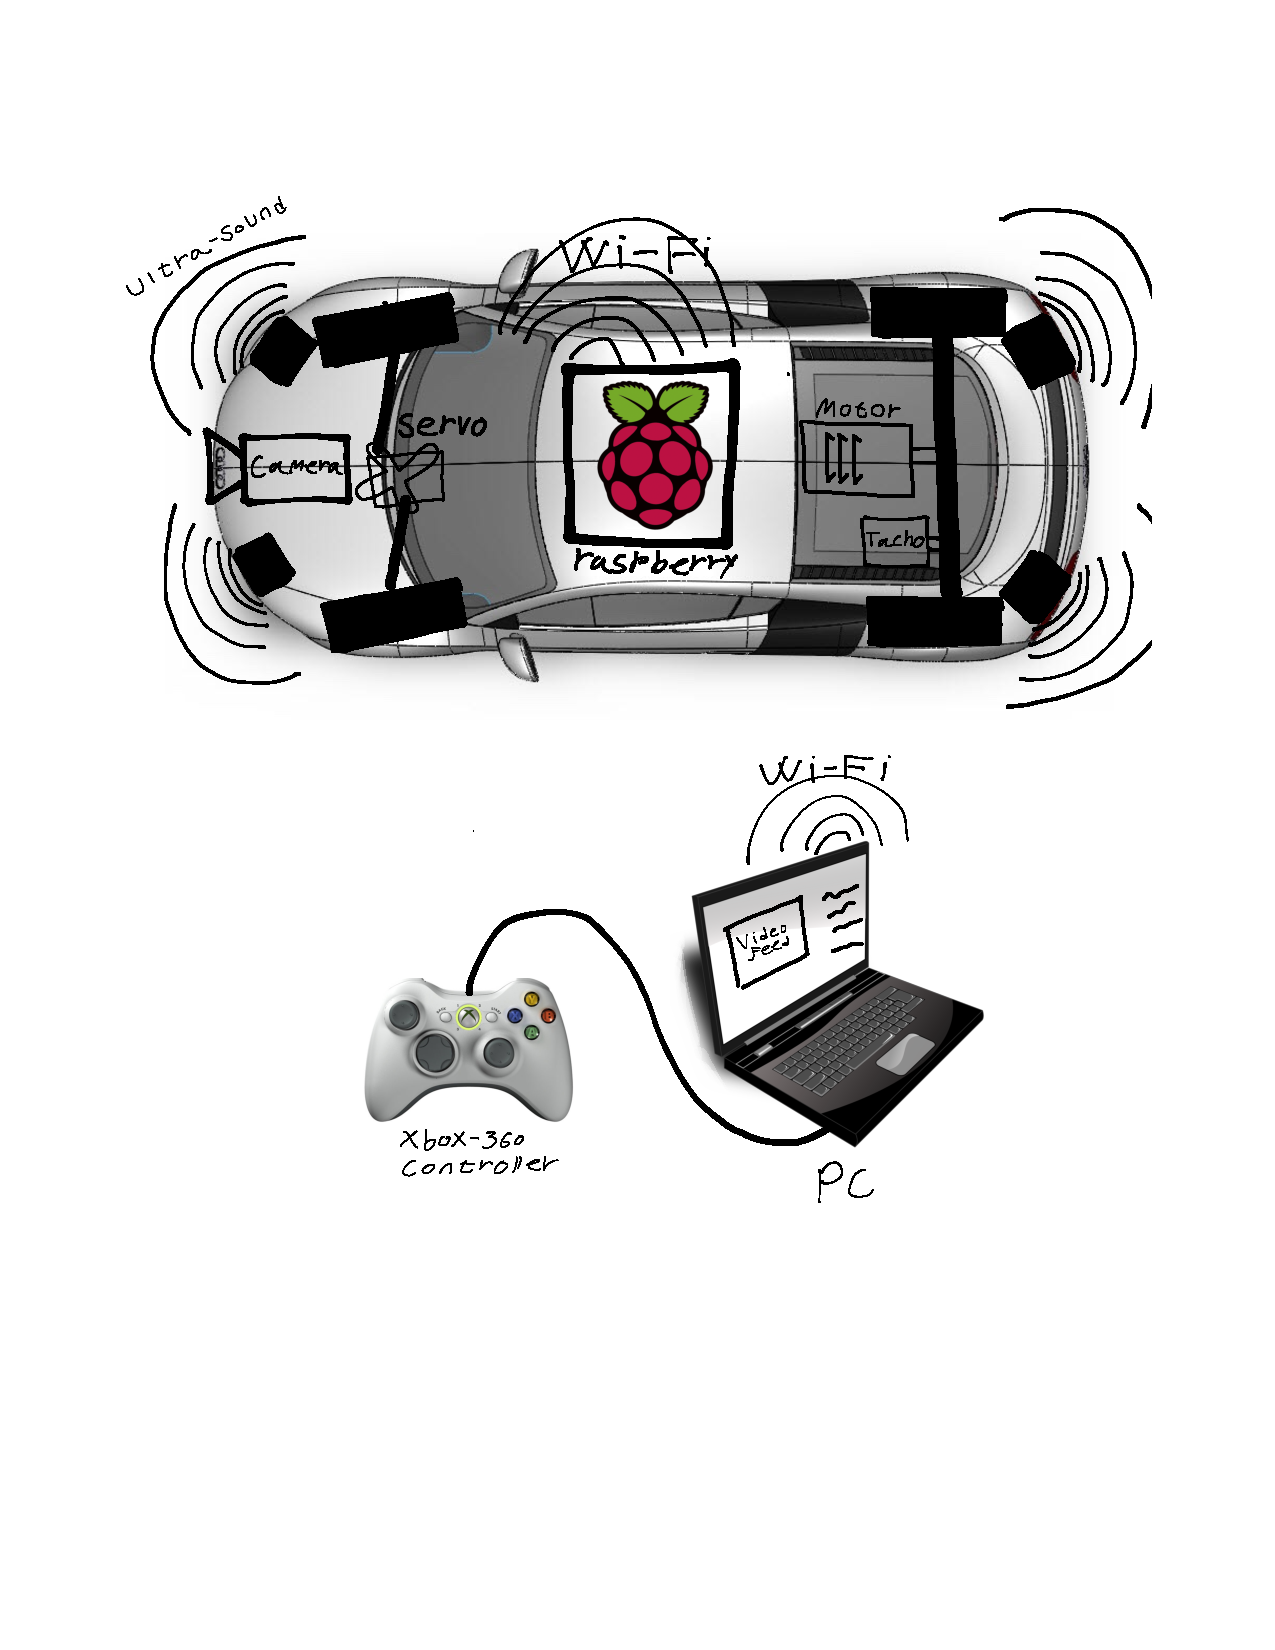
\includegraphics[width=\textwidth - 7.38 cm]{../fig/billeder/rigbillede}
\caption{Rigt billede af systemet i sin helhed}
\label{fig:rigbillede}
\end{figure}

%---------------------------------------------------------------------------------------
%											ORDBESKRIVELSE
%---------------------------------------------------------------------------------------

%==================== Ordforklaring ====================

\section{Ordforklaring}

\subsubsection{System}
Det totale system, indeholdende både bil, software på PC og netværkskommunikation mellem Bil og PC. 

\subsubsection{Human Interface Device (HID)}
En måde at kommunikere med en computer fx et tastatur, eller for dette projekts tilfælde, en XBOX360 controller.

\begin{itemize}
	\item Right Trigger (RT) - ??
	\item Left Trigger (LT) - ??
	\item Flere knapper her.
	%TODO list alle knapper på XBOX controller
\end{itemize}

\subsubsection{Hovedmenu}
Hovedmenuen i software på PC, indeholder menupunkter, som brugeren kan navigere efter behov.

\subsubsection{Bil}
Køretøjet samt controller som udfører alle relevante opgaver for bilen. Alt kommunikation med PC, foregår gennem denne.

\subsubsection{Wi-Fi}
Trådløst netværk af specifikationerne ''IEEE 802.11'', som Bil og PC kommunikerer over.

\subsubsection{Anti-kollitionssystem (AKS)}
Et system på bilen bestående af fire ultralydssensorer, som er i stand til at forhindre en kollision ved at overtage styringen fra Bruger i tilfælde af en kollisionskurs. Der gøres forskel mellem "Aktiver AKS" og "Tænd/Sluk AKS".

\begin{itemize}
	\item Tænd/Sluk bruges i forbindelse med at slå AKS fra eller til, således bilen ikke vil undgå en kollision hvis slukket, men vil undgå en kollsion hvis tændt. 
	\item AKS aktiveres ifm. at bilen er på vej til at kollidere med en forhindring, hvorefter bilen vil forhindre en kollision (AKS tændt) eller ej (AKS slukket).
\end{itemize}

\subsubsection{Ultralydssensorer}
Ultralydssensorerne benævnes herefter som hhv. Front Left (FL), Front Right (FR), Rear Left (RL) og Rear Right (RR). 

\clearpage 					 \cleartorightpage \cleartorightpage
%==================== Ordforklaring ====================

\section{Ordforklaring}

\subsubsection{System}
Det totale system, indeholdende både bil, software på PC og netværkskommunikation mellem Bil og PC. 

\subsubsection{Human Interface Device (HID)}
En måde at kommunikere med en computer fx et tastatur, eller for dette projekts tilfælde, en XBOX360 controller.

\begin{itemize}
	\item Right Trigger (RT) - ??
	\item Left Trigger (LT) - ??
	\item Flere knapper her.
	%TODO list alle knapper på XBOX controller
\end{itemize}

\subsubsection{Hovedmenu}
Hovedmenuen i software på PC, indeholder menupunkter, som brugeren kan navigere efter behov.

\subsubsection{Bil}
Køretøjet samt controller som udfører alle relevante opgaver for bilen. Alt kommunikation med PC, foregår gennem denne.

\subsubsection{Wi-Fi}
Trådløst netværk af specifikationerne ''IEEE 802.11'', som Bil og PC kommunikerer over.

\subsubsection{Anti-kollitionssystem (AKS)}
Et system på bilen bestående af fire ultralydssensorer, som er i stand til at forhindre en kollision ved at overtage styringen fra Bruger i tilfælde af en kollisionskurs. Der gøres forskel mellem "Aktiver AKS" og "Tænd/Sluk AKS".

\begin{itemize}
	\item Tænd/Sluk bruges i forbindelse med at slå AKS fra eller til, således bilen ikke vil undgå en kollision hvis slukket, men vil undgå en kollsion hvis tændt. 
	\item AKS aktiveres ifm. at bilen er på vej til at kollidere med en forhindring, hvorefter bilen vil forhindre en kollision (AKS tændt) eller ej (AKS slukket).
\end{itemize}

\subsubsection{Ultralydssensorer}
Ultralydssensorerne benævnes herefter som hhv. Front Left (FL), Front Right (FR), Rear Left (RL) og Rear Right (RR). 

\clearpage \cleartorightpage
\chapter{Kravspecifikation}
\section{Aktør-kontekstdiagram}

\begin{figure}[h]
\centering
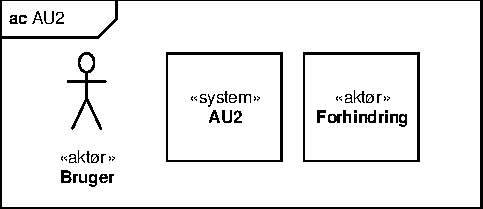
\includegraphics[width=\textwidth - 3 cm]{../fig/diagrammer/ac_au2.pdf}
\caption{Aktør kontekst diagram for AU2.}
\label{fig:aktor_kontekst}
\end{figure}

\section{Aktørbeskrivelser}
\subsubsection{Bruger - Primær Aktør}
Bruger kan:
\begin{itemize}
\item Starte og stoppe systemet 
\item Styre bilen over et netværk.
\item Deaktivere og aktivere anti-kollisionssystem.
\item (Vælge forskellige grader af anti-kollisionssystem??)
% Der menes her, at det skal være muligt at vælge imellem bremse- og styreting skal være aktivt eller ej.
\end{itemize}

\section{Funktionelle krav}
Systemet\ldots
\begin{enumerate}\itemsep1pt \parskip0pt \parsep0pt
	\item \ldots  \emph{Skal} kunne køre frem og tilbage.
	\item \ldots  \emph{Skal} kunne dreje.
	\item \ldots  \emph{Skal} kunne regulere hastigheden på bilen.
	\item \ldots  \emph{Skal} give Bruger mulighed for at begrænse maksimumshastighed.
	\item \ldots  \emph{Skal} give Bruger mulighed for manuel styring af hastighed og retning.
	\item \ldots  \emph{Skal} via Wi-Fi kunne kommunikere mellem bil og computer.
	\item \ldots  \emph{Skal} kunne identificere forhindringer foran og bag bilen.
	\item \ldots  \emph{Skal} indholde et anti-kollisionssystem baseret på afstandssensorer.
	\item \ldots  \emph{Skal} via. anti-kollisionssystemet kunne undvige og/eller stoppe før kollision.
	\item \ldots  \emph{Skal} indeholde et kamera til at streame video.
	\item \ldots  \emph{Bør} give Bruger mulighed for at aktivere/deaktivere anti-kollisionssystemet på bilen.
	\item \ldots  \emph{Kan} indeholde en batteriniveau-indikator.
\end{enumerate}

\section{Ikke-funktionelle krav}
\begin{enumerate}
	\item Bilens maksimumshastighed uden begrænsning er 20km/t $\pm$ 5\% %TODO Passer denne?
	\item Bilens bremselængde ved maksimumshastighed uden begrænsning må ikke overstige 1 m. %TODO Passer denne?
	\item Bilen skal kunne accelerere fra 0 km/t til maksimumshastighed uden begrænsning på højest 6 s. %TODO Passer denne?
	\item Forsinkelse fra brugerinput til at bilen reagerer må ikke overstige 50ms. %TODO Passer denne?
	\item Afstandssensorerne skal kunne identificere en forhindring på mindst $(30cm \times 30cm)$ på en maksimal afstand af 6 m. %TODO Passer denne, EMC - spørg vejleder?
	\item Mister bilen forbindelsen med computeren i mere end 50ms, standser bilen automatisk. 
	\item Kameraet skal minimum have en opdateringshastighed på 15 billeder i sekundet. %TODO undersøg!
	\item Systemet skal vise video-feed med en opløsning på $640 \times 480$ pixels.
	\item Computeren skal som minimum sende kommandoer til bilen 60 gange i sekundet. 
	\item HID skal bestå af en XBOX360 controller og tastatur.
\end{enumerate}

\newpage
\section{Use Cases}



% UC1:  Aktiver system
\newpage
\begin{longtable}{| l | >{\raggedright}X | >{\raggedright}X | >{\raggedright}X | >{\raggedright\arraybackslash}p{2.3cm} |} \hline
	\multicolumn{2}{|l|}{\textbf{Use case under test}} & 
	\multicolumn{3}{l|}{UC1: Aktiver system} \\ \hline
	
	\multicolumn{2}{|l|}{\textbf{Scenarie}} & 
	\multicolumn{3}{l|}{Hovedscenarie} \\ \hline
	
	\multicolumn{2}{|l|}{\textbf{Forudsætning}} & 
	\multicolumn{3}{p{10.2cm}|}{Netværksforbindelse er opsat og fungerende\hfill} \\ \hline
	%\multicolumn{5}{|l|}{}\\ \hline
	\textbf{Step} & \textbf{Handling} & \textbf{Forventet Resultat} & \textbf{Resultat} & \textbf{Godkendt / Kommentar} \\ \hline

	1.1 & Bruger sætter bilens ''ON/OFF''-switch til ''ON''. 
		& Visuel test:\\ Lampe på bilens strømforsyning lyser.
		& Lampen lyser ikke, strømforsyning kan høres. Pi og PSoC starter op og deres respektive LEDer lyser.
		& IKKE OK - Forsyning til lampe på strømforsyningen er ikke forbundet.\\ \hline
		
	1.2 & Bruger starter software på PC.
		& Visuel test:\\ Hovedvinduet vises på skærmen.
		& Hovedvinduet ses på skærmen
		& OK\\ \hline
		
	1.3 & Bruger trykker på ''Opret forbindelse''.
		& Visuel test:\\ Hovedvindue viser ''Forbindelse oprettet''.
		& En pop-op med forbindelse oprettet vises
		& OK\\ \hline
		
	1.4 & Bruger observerer hovedvinduet.
		& Visuel test:\\ Videostream vises i hovedvinduet.
		& Videostream kan ses i hovedvinduet
		& OK\\ \hline
		
	1.5 & Bruger observerer hovedvinduet.
		& Visuel test:\\ Bilens aktuelle hastighed vises i hovedvinduet.
		& Bilens hastighed vises i hovedvinduet, opdateres dog ikke hvis bilen står stille (viser ej 0 km/t)
		& OK\\ \hline
		
	1.6 & Bruger observerer hovedvinduet.
		& Visuel test:\\ Bilens aktuelle tyngdeacceleration vises i hovedvinduet.
		& Acceleration G opdateres ikke
		& IKKE OK - Accelerometer er ikke implementeret.\\ \hline
		
	1.7 & Bruger observerer hovedvinduet.
		& Visuel test:\\ Data fra bilens afstandssensorer vises i hovedvinduet.
		& Hovedvinduet viser korteste afstand for sensorerne i meter - ikke præcis over 1m
		& OK\\ \hline
		
\caption{Accepttest for UC1: Aktiver system}\label{tbl:acceptuc1}
\end{longtable}

% UC2: Stream Videofeed
\newpage
\begin{longtable}{| l | >{\raggedright}X | >{\raggedright}X | >{\raggedright}X | >{\raggedright\arraybackslash}p{2.3cm} |} \hline
	\multicolumn{2}{|l|}{\textbf{Use case under test}} & 
	\multicolumn{3}{l|}{UC2: Stream Video} \\ \hline
	
	\multicolumn{2}{|l|}{\textbf{Scenarie}} & 
	\multicolumn{3}{l|}{Hovedscenarie} \\ \hline
	
	\multicolumn{2}{|l|}{\textbf{Forudsætning}} & 
	\multicolumn{3}{p{10.2cm}|}{UC1 frem til punkt 5 er fuldført \hfill} \\ \hline
	%\multicolumn{5}{|l|}{}\\ \hline
	\textbf{Step} & \textbf{Handling} & \textbf{Forventet Resultat} & \textbf{Resultat} & \textbf{Godkendt / Kommentar} \\ \hline

	2.1 & Bruger åbner AU2 softwaren på PC'en og trykker ''Opret forbindelse''. %TODO: Dobbelttjek navngivning her.
		& Visuel test:\\ Der vises et live-feed fra bilens kamera.
		& Videostream kan ses i hovedvinduet.
		& OK\\ \hline
	2.2 & Bruger har Wireshark åbent på samme computer. Wireshark er opsat til at overvåge det pågældene netværk.
		& Visuel test:\\ I Wireshark observeres der for overføring af pakker fra bilens IP-adresse til computerens IP-adresse.
		& Der overføres pakker fra Pi til computeren.
		& OK\\ \hline
		
\caption{Accepttest for UC2: Stream Video}\label{tbl:acceptuc2}
\end{longtable}

% UC3: Overvåg sensor
\newpage
\subsubsection{Use Case 3: Overvåg sensor}

%-------------------- UC3 --------------------
\begin{table}[h]
\begin{tabularx}{\textwidth}{| >{\raggedright\arraybackslash}p{3.3 cm} | >{\raggedright\arraybackslash}X |} \hline

\textbf{Navn:} 						 & UC3: Overvåg sensorer				\\ \hline
\textbf{Mål:}						 & At overvåge sensorer 				\\ \hline
\textbf{Initiering:}				 & UC1: Aktiver system 					\\ \hline
\textbf{Aktører:} 					 & Ingen 								\\ \hline
\textbf{Reference:} 				 & UC1, UC4: Undvig forhindring,UC9: Tænd/sluk AKS	\\ \hline
\textbf{Antal samtidige forekomster:}& Én 									\\ \hline
\textbf{Forudsætning:} 				 & UC1 frem til punkt 7 er fuldført		\\ \hline
\textbf{Resultat:}					 & Sensorer overvåges løbende  			\\ \hline
\textbf{Hovedscenarie:}				 & 

\begin{packed_enum}
	\item Bilen initierer tachometer
		\begin{packed_item}\itemsep1pt \parskip0pt \parsep0pt
			\item {[}Ext 1.a: Initiering af tachometer fejler{]}
		\end{packed_item}
	\item Bilen initierer accelerometer
		\begin{packed_item}\itemsep1pt \parskip0pt \parsep0pt
			\item {[}Ext 2.a: Initiering af accelerometer fejler{]}
		\end{packed_item}
	\item Bilen initierer afstandssensorer.
		\begin{packed_item}\itemsep1pt \parskip0pt \parsep0pt
			\item {[}Ext 3.a: Initiering af afstandssensorer fejler{]}
		\end{packed_item}
	\item Bilen overvåger sensorer.
	\item UC4: Undvig forhindring initieres af System
	\begin{packed_item}\itemsep1pt \parskip0pt \parsep0pt
			\item {[}Ext 5.a: AKS er slukket via UC9: Tænd/sluk AKS{]}
		\end{packed_item}
	\item Bilen modtager data fra PC.
	\item Bilen sender sensor data til PC.
\end{packed_enum} 															\\ \hline

\textbf{Udvidelser:}				&  
\textbf{{[}Ext 1.a : Initiering af tachometer fejler{]}}
	\begin{packed_enum}\itemsep1pt \parskip0pt \parsep0pt
		\item Systemet prompter PC med ''tachometer-initiering fejlet''.
		\item UC2 afsluttes.
	\end{packed_enum}	
														
\textbf{{[}Ext 2.a : Initiering af accelerometer fejler{]}}
	\begin{packed_enum}\itemsep1pt \parskip0pt \parsep0pt
		\item Systemet prompter PC med ''accelerometer-initiering fejlet''.
		\item UC2 afsluttes.
	\end{packed_enum}
	
\textbf{{[}Ext 3.a : Initiering af afstandssensorer fejler{]}}
	\begin{packed_enum}\itemsep1pt \parskip0pt \parsep0pt
		\item Systemet prompter PC med ''afstandssensor-initiering fejlet''.
		\item UC2 afsluttes.
	\end{packed_enum}
	
	\textbf{{[}Ext 5.a : AKS er slukket via UC9: Tænd/sluk AKS{]}}
	\begin{packed_enum}\itemsep1pt \parskip0pt \parsep0pt
		\item Use casen fortsætter fra punkt 6.
	\end{packed_enum}														\\\hline

\end{tabularx}
\caption{UC3: Overvåg sensorer}
\label{tbl:UC3}
\end{table}

% UC4: Aktiver AKS
\newpage

\begin{longtable}{| l | >{\raggedright}X | >{\raggedright}X | >{\raggedright}X | >{\raggedright\arraybackslash}p{2.3cm} |} \hline
	\multicolumn{2}{|l|}{\textbf{Use case under test}} & \multicolumn{3}{l|}{UC4: Undvig forhindring} \\ \hline
	\multicolumn{2}{|l|}{\textbf{Scenarie}} & \multicolumn{3}{l|}{Hovedscenarie} \\ \hline
	\multicolumn{2}{|l|}{\textbf{Forudsætning}} & \multicolumn{3}{p{10.2cm}|}{UC1 er gennemført, UC3 er gennemført.\hfill} \\ \hline
	%\multicolumn{5}{|l|}{}\\ \hline
	\textbf{Step} & \textbf{Handling} & \textbf{Forventet Resultat} & \textbf{Resultat} & \textbf{Godkendt / Kommentar} \\ \hline
	
	4.1 & Bruger styrer bilen fremad mod en forhindring på min. $(30cm \times 30cm)$ vinkelret på bilens kørebane vha. Xbox-360 controlleren, således at bilen er umiddelbart til venstre for objektet. & Visuel test: \\ Bruger observerer at bilen ændrer kurs til højre på trods af brugerinput. & ~ & ~ \\ \hline
	
	4.2 & Bruger tester om det er muligt at styre bilen igen med Xbox-360 controlleren. & Visuel test: \\ Bruger observerer at bilen reagerer på brugerinput. & ~  & ~ \\ \hline
	
	4.3 & Bruger styrer bilen fremad mod en forhindring på $(30cm \times 30cm)$ vinkelret på bilens kørebane vha. Xbox-360 controlleren, således at bilen er umiddelbart til højre for objektet. & Visuel test: \\ Bruger observerer at bilen ændrer kurs til venstre på trods af brugerinput. & ~ & ~\\ \hline
	
	4.4 & Bruger styrer bilen fremad mod en forhindring på $(30cm \times 30cm)$ vinkelret på bilens kørebane vha. Xbox-360 controlleren, således at bilen har retning lige mod objektet. & Visuel test: \\ Bruger observerer at bilen standser på trods af brugerinput. & ~ & ~ \\\hline
	
	4.5 & Bruger bakker mod en forhindring på $(30cm \times 30cm)$ vinkelret på bilens kørebane vha. Xbox-360 controlleren, således at bilen er umiddelbart til venstre for objektet. & Visuel test: \\ Bruger observerer at bilen ændrer kurs til venstre på trods af brugerinput. & ~ & ~ \\ \hline
	
	4.6 & Bruger bakker bilen mod en forhindring på $(30cm \times 30cm)$ vinkelret på bilens kørebane vha. Xbox-360 controlleren, således at bilen er umiddelbart til højre for objektet. & Visuel test: \\ Bruger observerer at bilen ændrer kurs til højre på trods af brugerinput. & ~ & ~\\ \hline
	
	4.7 & Bruger bakker bilen mod en forhindring på $(30cm \times 30cm)$ vinkelret på bilens kørebane vha. Xbox-360 controlleren, således at bilen har retning lige mod objektet. & Visuel test: \\ Bruger observerer at bilen standser på trods af brugerinput. & ~ & ~\\\hline

\caption{Accepttest for UC4: Undvig forhindring}\label{tbl:acceptuc4}
\end{longtable}

% UC5: Kør bil frem/tilbage
\newpage
\subsection{Use Case 5: Kør bil frem/tilbage}
\begin{table}[h]
\begin{tabularx}{\textwidth}{| L{3.3 cm} | Z |} \hline

\textbf{Navn:} 						& UC5: Kør bil frem/tilbage\\ \hline
\textbf{Mål:}						& At få bilen til at køre frem eller tilbage. \\ \hline
\textbf{Initiering:}				& Bruger \\ \hline
\textbf{Aktører:} 					& Bruger \\ \hline
\textbf{Reference:} 				& Ingen \\ \hline
\textbf{Antal samtidige forekomster:} & Én \\ \hline
\textbf{Forudsætning:} 				& UC1: Aktiver system er fuldført og systemet er operationelt. \\ \hline
\textbf{Resultat:}					& Bilens hastighed er ændret. \\ \hline
\textbf{Hovedscenarie:}				& 

\begin{packed_enum}
\item Bruger ændrer position af RT på HID controlleren.
	\begin{packed_item}\itemsep1pt \parskip0pt \parsep0pt
	\item {[}Ext 1.a: Bruger ændrer position af LT.{]}
	\end{packed_item}
\item Controllerens input streames til bilen.
\item Bilen ændrer fremadgående hastighed i henhold til brugerens input. Et hårdere tryk resulterer i en højere hastighed og et lettere tryk resulterer i en lavere hastighed.
\item UC5 afsluttes.
\end{packed_enum} \\ \hline
\textbf{Udvidelser:}				&  
\textbf{{[}Ext 1.a : Bruger ændrer position af LT.{]}}
	\begin{packed_enum}\itemsep1pt \parskip0pt \parsep0pt
		\item Controllerens input streames til bilen.
		\item Bilen ændrer bagudgående hastighed i henhold til brugerens input. Et hårdere tryk resulterer i en højere hastighed og et lettere tryk resulterer i en lavere hastighed.
		\item Systemet fortsætter fra punkt 4 i hovedscenariet.
	\end{packed_enum}
\\ \hline
\end{tabularx}
\caption{UC5: Kør bil frem/tilbage}
\label{tbl:UC5}
\end{table}

% UC6: Drej bil til højre/Venstre
\newpage
\subsection{Use Case 6: Drej bil til højre/venstre}
\begin{table}[h]
\begin{tabularx}{\textwidth}{| L{3.3 cm} | Z |} \hline

\textbf{Navn:} 						& UC6: Drej til højre/venstre\\ \hline
\textbf{Mål:}						& At få bilen til at dreje mod højre eller venstre. \\ \hline
\textbf{Initiering:}				& Bruger \\ \hline
\textbf{Aktører:} 					& Bruger eller AKS \\ \hline
\textbf{Reference:} 				& Ingen\\ \hline
\textbf{Antal samtidige forekomster:} & Én \\ \hline
\textbf{Forudsætning:} 				& UC1: Aktiver system er fuldført og systemet er operationelt. \\ \hline
\textbf{Resultat:}					& Retningen på bilens forhjul er ændret. \\ \hline
\textbf{Hovedscenarie:}				& 

\begin{packed_enum}
\item Bruger ændrer position på den venstre styrepind på HID controlleren.
	\begin{packed_item}\itemsep1pt \parskip0pt \parsep0pt
	\item {[}Ext 1.a: AKS er aktiveret.{]}
	\end{packed_item}
\item Controllerens input streames til bilen.
\item Bilen tjekker input, hvis den er mere mod venstre drejer hjulet mere til venstre og omvendt. %TODO dette skal lige finpudses lidt.
\item UC6 afsluttes.
\end{packed_enum} \\ \hline
\textbf{Udvidelser:}				&  
\textbf{{[}Ext 1.a : AKS er aktiveret.{]}}
	\begin{packed_enum}\itemsep1pt \parskip0pt \parsep0pt
		\item Bilen analyserer input fra UC3.
		\item Bilen drejer til højre, hvis sensor FL registrerer en forhindrer, ditto venstre og FR.
		\item Bilen undviger forhindringen. %TODO Skal eventuelt lige finpudses
		\item Systemet fortsætter fra punkt 3 i hovedscenariet.
	\end{packed_enum}
\\ \hline
\end{tabularx}
\caption{UC6: Drej til højre/venstre}
\label{tbl:UC6}
\end{table}

% UC7: Brems bil %TODO
\newpage
\begin{longtable}{| l | >{\raggedright}X | >{\raggedright}X | >{\raggedright}X | >{\raggedright\arraybackslash}p{2.3cm} |} \hline
	\multicolumn{2}{|l|}{\textbf{Use case under test}}  & \multicolumn{3}{l|}{UC7: Brems Bil} \\ \hline
	\multicolumn{2}{|l|}{\textbf{Scenarie}} 			& \multicolumn{3}{l|}{Hovedscenarie} \\ \hline
	\multicolumn{2}{|l|}{\textbf{Forudsætning}} 		& \multicolumn{3}{p{10.2cm}|}{UC1: Aktiver system er fuldført og systemet er operationelt.\hfill} \\ \hline
	%\multicolumn{5}{|l|}{}\\ \hline
	\textbf{Step} 	& \textbf{Handling} & \textbf{Forventet Resultat} & \textbf{Resultat} & \textbf{Godkendt / Kommentar} \\ \hline
	7.1 & Bruger trykker på ''X'' knappen på Xbox-360 controlleren. 
		& Visuel test: Bruger observerer at bilens hastighed sænkes. 
		&   
		&  \\ \hline
	
\\ \hline
\caption{Accepttest for UC7: Brems Bil }\label{tbl:acceptuc7}
\end{longtable}

% UC8: Konfigurer system
\newpage
\subsection{Use Case 8: Konfigurer IP-adresse}
%-------------------- UC8 --------------------
\begin{table}[h]
\begin{tabularx}{\textwidth}{| >{\raggedright\arraybackslash}p{3.3 cm} | >{\raggedright\arraybackslash}X |} \hline

\textbf{Navn:} 						& UC8: Konfigurer IP-adresse										\\ \hline
\textbf{Mål:}						& At konfigurere bilens IP-adresse til PC'en						\\ \hline
\textbf{Initering:}					& Bruger 															\\ \hline
\textbf{Aktører:} 					& Bruger															\\ \hline
\textbf{Reference:} 				& Ingen																\\ \hline
\textbf{Antal samtidige forekomster:} & Én 																\\ \hline
\textbf{Forudsætning:} 				& UC1: Aktiver system er udført til punkt 3, 
									  bilen og PC er på samme netværk,systemet viser ''Hovedvindue'' 
									  samt at systemet er operationelt									\\ \hline
\textbf{Resultat:}					& IP adressen på bilen er indstillet								\\ \hline
\textbf{Hovedscenarie:}				& 

\begin{packed_enum}
	\item Bruger trykker på ''Konfigurer IP''.
	\item Konfigurationssmenuen for IP-adressen vises, og der er mulighed for at indtaste en IP-adresse.
	\item Bruger indtaster bilens IP-adresse.
	\item Bruger trykker ''Gem'' og system viser ''Hovedvindue''.
	\item Bruger trykker på ''Opret forbindelse''.
	\item Menuen indikerer at der er forbindelse til bilen.
	\begin{packed_item}\itemsep1pt \parskip0pt \parsep0pt
		\item {[}Ext 6.a Menuen indikerer at der ikke er forbindelse til bilen{]}
	\end{packed_item}
	\item Bruger trykker på ''Tilbage''.
	\item Systemet viser ''Hovedvindue''.
\end{packed_enum}																						\\ \hline
\textbf{Udvidelser:}				&  
\textbf{[}Ext 6.a Menuen indikerer at der ikke er forbindelse til bilen{]}
	\begin{packed_enum}\itemsep1pt \parskip0pt \parsep0pt
	\item Bruger gentager fra punkt 2 i hovedscenarie. 
	\end{packed_enum}																					\\ \hline
\end{tabularx}
\caption{UC8: Konfigurer IP-adresse}
\label{tbl:UC8}
\end{table}

\newpage
\subsection{Use Case 9: Tænd/sluk AKS}
%-------------------- UC9 --------------------
\begin{table}[h]
\begin{tabularx}{\textwidth}{| L{3.3 cm} | Z |} \hline

\textbf{Navn:} 						& UC9: Tænd/sluk AKS \\ \hline
\textbf{Mål:}						& At tænde eller slukke for AKS på bilen \\ \hline
\textbf{Initering:}					& Bruger \\ \hline
\textbf{Aktører:} 					& Bruger (primær) \\ \hline  
\textbf{Reference:} 					& UC11: Kalibrer system\\ \hline
\textbf{Antal samtidige forekomster:} & Én \\ \hline
\textbf{Forudsætning:} 				& UC1: Aktiver system er udført, bilen og PC er på samme netværk, at systemet viser ''Hovedmenu'' samt at systemet er operationelt\\ \hline
\textbf{Resultat:}					&  \\ \hline
\textbf{Hovedscenarie:}				& 

\begin{packed_enum}
\item Bruger trykker på ''AKS'' 
\item Menuen for AKS kommer frem og der er mulighed for at tænde/slukke for AKS 
\item Menuen indikerer om der er tændt/slukket for AKS
\item Bruger trykker tænd/sluk efter ønske
\item Bilen tænder/slukker for AKS systemet efter brugerens ønske
\item Menuen indikerer nuværende status af AKS
\end{packed_enum} \\ \hline
\textbf{Udvidelser:}				&  
~
\\ \hline
\end{tabularx}
\caption{UC9: Tænd/sluk AKS}
\label{tbl:UC9}
\end{table}

\newpage
\begin{longtable}{| l | >{\raggedright}X | >{\raggedright}X | >{\raggedright}X | >{\raggedright\arraybackslash}p{2.3cm} |} \hline
	\multicolumn{2}{|l|}{\textbf{Use case under test}}  & \multicolumn{3}{l|}{UC10: Indstil makshastighed} \\ \hline
	\multicolumn{2}{|l|}{\textbf{Scenarie}} 			& \multicolumn{3}{l|}{Hovedscenarie} \\ \hline
	\multicolumn{2}{|l|}{\textbf{Forudsætning}} 		& \multicolumn{3}{p{10.2cm}|}{UC1: Aktiver system er udført, bilen og PC er på samme netværk, at systemet viser ''Hovedvindue'' samt at systemet er operationelt.\hfill} \\ \hline
	%\multicolumn{5}{|l|}{}\\ \hline
	\textbf{Step} 	& \textbf{Handling} & \textbf{Forventet Resultat} & \textbf{Resultat} & \textbf{Godkendt / Kommentar} \\ \hline
	
	10.1 & Bruger trykker på ''Indstil makshastighed''. 
		 & Visuel test: \\ Hovedvindue viser menu med mulighed for at indtaste makshastighed fra 1-10 km/t. 
		 & Vindue med mulighed for indstilling af max hastighed vises.
		 & OK\\ \hline
	10.2 & Menuen viser bilens nuværende makshastighed. 
		 & Den nuværende makshastighed vises.
		 & Den nuværende makshastighed vises til højre.
		 & OK\\ \hline
	10.3 & Bruger indtaster bilens ønskede makshastighed. 
		 & Menuen viser den ønskede makshastighed. 
		 & Der vises den nye makshastighed 
		 & OK\\ \hline
	10.4 & Bruger trykker på ''Ok''. 
		 & Systemet viser den nye makshastighed. 
		 & Systemet viser den indstillede makshastighed
		 & OK\\ \hline
	10.5 & Bruger holder ''RT'' inde på Xbox 360 controlleren.
		 & Bilen accelerer til den angivne maksimalhastighed.
		 & Bilen ændrer makshastighed ift. den indtastede, dette er dog ikke målt præcist
		 & MÅSKE OK\\ \hline
		 
\caption{Accepttest for UC10: Indstil makshastighed }\label{tbl:acceptuc10}
\end{longtable}

% UC11: Kalibrer system
\newpage
\subsection{Use Case 11: Kalibrer styretøj}
%-------------------- UC11 --------------------
\begin{table}[h]
\begin{tabularx}{\textwidth}{| >{\raggedright\arraybackslash}p{3.3 cm} | >{\raggedright\arraybackslash}X |} \hline

\textbf{Navn:} 						& UC11: Kalibrer styretøj												\\ \hline
\textbf{Mål:}						& At kalibrere systemet så bilen kører ligeud 
									  når brugeren slipper styrepinden på Xbox-360 controlleren 			\\ \hline
\textbf{Initering:}					& Bruger 																\\ \hline
\textbf{Aktører:} 					& Bruger																\\ \hline
\textbf{Reference:} 			    & Ingen																	\\ \hline
\textbf{Antal samtidige forekomster:} & Én 																	\\ \hline
\textbf{Forudsætning:} 				& UC1: Aktiver system er udført, bilen og PC er på samme netværk, 
									  at systemet viser ''Hovedmenu'', at systemet er operationelt 
									  samt bilen holder stille												\\ \hline
\textbf{Resultat:}					& Bilens styretøj er kalibreret 										\\ \hline
\textbf{Hovedscenarie:}				& 

\begin{packed_enum}
	\item Bruger vælger ''Kalibrer styretøj''.
	\item Systemet viser menu for Kalibrering med mulighed for indtastning af værdi mellem -50 og 50. %TODO dette tal skal evt. rettes
	\item Bruger indtaster værdi. 
	\begin{packed_item}\itemsep1pt \parskip0pt \parsep0pt
		\item {[}Ext 3.a : Bruger indtaster ugyldig værdi{]} %TODO mellemrum mellem bogstav og :? Husk at rette i alle UC
	\end{packed_item}
	\item Bruger trykker på ''Gem''.
	\item Systemet gemmer værdien på bilen.
	\item Forhjulene drejer en absolut værdi mod enten, højre eller venstre: positiv værdi oversætte til højre, og negativ værdi oversættes venstre.
	\item Systemet returnerer til ''Hovedvindue''
\end{packed_enum} 																							\\ \hline
\textbf{Udvidelser:}					&  
\textbf{[}Ext 3.a : Bruger indtaster en ugyldig værdi{]}
	\begin{packed_enum}\itemsep1pt \parskip0pt \parsep0pt
		\item Systemet prompter: ''Ugyldig værdi, indtast en gyldig værdi.''
		\item Systemet fortsætter fra punkt 2 i hovedscenariet.
	\end{packed_enum}																						\\ \hline
\end{tabularx}
\caption{UC11: Kalibrer styretøj}
\label{tbl:UC11}
\end{table}

% UC12: Afbryd system
\newpage 
\begin{longtable}{| l | >{\raggedright}X | >{\raggedright}X | >{\raggedright}X | >{\raggedright\arraybackslash}p{2.3cm} |} \hline
	\multicolumn{2}{|l|}{\textbf{Use case under test}} & 
	\multicolumn{3}{l|}{UC12: Afbryd system} \\ \hline
	
	\multicolumn{2}{|l|}{\textbf{Scenarie}} & 
	\multicolumn{3}{l|}{Hovedscenarie} \\ \hline
	
	\multicolumn{2}{|l|}{\textbf{Forudsætning}} & 
	\multicolumn{3}{p{10.2cm}|}{UC1: Aktiver system er fuldført, bilen holder stille og systemet er operationelt\hfill} \\ \hline
	%\multicolumn{5}{|l|}{}\\ \hline
	\textbf{Step} & \textbf{Handling} & \textbf{Forventet Resultat} & \textbf{Resultat} & \textbf{Godkendt / Kommentar} \\ \hline

	12.1 & Bruger lukker ned for softwaren på PC'en. 
		 & Visuel test:\\ Hovedvinduet forsvinder fra skærmen.
		 & 
		 & \\ \hline
		
	12.2 & Bruger skubber kontakten ''ON/OFF'' på undersiden af bilen til position ''OFF''
		 & Visuel test:\\ Lampe på strømforsyning slukker.
	 	 & 
		 & \\ \hline
		
\caption{Accepttest for UC12: Afbryd system}\label{tbl:acceptuc12}
\end{longtable} \cleartorightpage
%\section{Systemarkitektur}
\label{ch:Systemarkitektur}

%TODO
OBS: Stjålet fra PRJ3

I systemarkitekturen beskrives grænseflader for systemet og hvilke blokke det består af. Til at beskrive dette er der anvendt en række BDD'er og IBD'er. Nedenfor er de vigtigste af disse vist. For mere detaljeret beskrivelse se afsnit \ref{P-ch:SysArk} \nameref{P-ch:SysArk} på side \pageref{P-ch:SysArk} i projektdokumentationen.

her var et overordnet bdd for system


På Figur \ref{fig:bdd_system} kan der skabes et overblik over systemet og hvilke underblokke det består af. Det kan ses, at systemet består af syv underblokke, bl.a. PSoC Master, DevKit8000 mm. I blokken System, der består af alle de andre underblokke, vises de porte som hele systemet har, dvs. grænsefladen til omverdenen.

\clearpage

her var et IBD over signaler

På Figur \ref{fig:ibd_system_signal} vises alle signalerne i systemet, dvs. alle spændingsforsyninger og referencer er udeladt for overskuelighedens skyld. For at beskrive de interne signaler, tages der udgangspunkt i DevKit8000. DevKit8000 spørger løbende PSoC Master om temperatur, luftfugtighed, lysintensitet samt jordfugtighed over UART, denne er detaljeret beskrevet på side \pageref{P-sec:UART_protokol} i projektdokumentationen. Kommunikationen mellem PSoC Master, Jordfugt, Temp/Luftfugtighed, Lyssensor og Aktuator foregår over en \IIC bus. Via denne kommunikationsvej kan PSoC Master'en efterspørge alle sensorværdierne og aktivere aktuatorer, hvis DevKit8000 ønsker at regulere klimaet i drivhuset med varmelegemet, vinduet og/eller blæserne. Der kan ses en signalbeskrivelse, hvor alle signaler mellem hver blok er beskrevet i Tabel \ref{P-tbl:signalbeskriv} på side \pageref{P-tbl:signalbeskriv} i dokumentationen.

\clearpage

her var et UML diagram for au2green

På Figur \ref{fig:UML} ses et UML klassediagram, som viser relationer mellem klasserne på DevKit8000. Der anvendes to relationstyper; komposition og association. Domain klassen datalog har til opgave at gemme de sensordata som monitor opsamler, jf. Listing \ref{P-lst:Sensordata_struct} på side \pageref{P-lst:Sensordata_struct} i dokumentationen. Regulatoren anvender denne information og bruger den til at afgøre, om forholdene i drivhuset er som ønsket. DevKit8000 er som angivet en controller klasse, og derfor binder den de øvrige klasser sammen og har den overordnede styring.

\clearpage

her var en figur over menuer 

Menuoversigten, der ses på Figur \ref{fig:QTMenu}, gives et samlet overblik over hvordan de forskellige menuer tilgås igennem systemet. Systemet viser altid hovedmenuen, når systemet starter op. Herfra er det muligt at få et overblik over drivhusets aktuelle klima. Hovedmenuen viser desuden fem knapper, hvor man kan få adgang til undermenuerne: virtuel drivhus-, historik-, plantedatabase-, systemlog- og konfigurationsmenu.

\clearpage \cleartorightpage
%\include{hardwareDesign/HardwareDesign} \cleartorightpage
%\include{softwareDesign/SoftwareDesign} \cleartorightpage
%\include{hardwareImplementering/HardwareImplementering} \cleartorightpage
%\section{Software Implementering} \label{ch:SWimplementering}

%TODO
write me %NEVER!

\clearpage \cleartorightpage
%\chapter{Accepttest} \label{ch:Accepttest}
\section*{Version}
\begin{table}[h]
	\centering
	\begin{tabularx}{\textwidth - 2cm}{|l|l|l|X|}
	\hline
	Dato			& Version			& Initialer 		& Ændring										\\ \hline
	29 September 	& 1 				& Alle				& Første udkast. 								\\ \hline
	 				& 2 				&  					& 						 						\\ \hline
			 		& 3 				&  					& 												\\ \hline
					& 4 				&  					& 												\\ \hline
	\end{tabularx}
\end{table}
\clearpage

\section{Funktionelle Krav}
%Her vælges bredde på hele tabellen samt hvilken FIL selve tabellen defineres i.
\LTXtable{\textwidth}{accepttest/uc1}
\LTXtable{\textwidth}{accepttest/uc2}
\clearpage
\LTXtable{\textwidth}{accepttest/uc3} 
\clearpage
\LTXtable{\textwidth}{accepttest/uc4}
\clearpage
\LTXtable{\textwidth}{accepttest/uc5} 
\clearpage
\LTXtable{\textwidth}{accepttest/uc6}
\LTXtable{\textwidth}{accepttest/uc7}
\clearpage
\LTXtable{\textwidth}{accepttest/uc8}
\LTXtable{\textwidth}{accepttest/uc9}
\clearpage
\LTXtable{\textwidth}{accepttest/uc10}
\LTXtable{\textwidth}{accepttest/uc11}
\LTXtable{\textwidth}{accepttest/uc12}

\clearpage

\section{Ikke-funktionelle krav}
\LTXtable{\textwidth}{Accepttest/ikke_funk}

\clearpage
%\renewcommand{\bibname}{Litteraturliste}
\fancyhead[CE,CO]{}
\fancyfoot[CE,CO]{}
\begin{thebibliography}{2}

%SKABELON*** \bibitem{lib:##REF##} ##FIRMANAVN##: \textit{##FORKLARING##}. \\ ##\URL{} ELLER BILAG XXX??##. ##DATO##

\bibitem {lib:MIPICSI-2} Mipi Alliance: \textit{Kamera interface standard}. \\ 
\url{http://mipi.org/specifications/camera-interface}. 2015.

\bibitem {lib:PI2PSU} RASPBERRY PI FOUNDATION: \textit{Anbefalet PSU størrelse}. \\
\url{https://www.raspberrypi.org/help/faqs/#powerReqs}. 2015.

\bibitem {lib:maxsonar} MaxBotix: \textit{I2CXL-MaxSonar-EZ0 datablad}. \\
\url{http://www.maxbotix.com/Ultrasonic_Sensors/MB1202.htm}. 2015.

\bibitem {lib:servo} Corona: \textit{CS238MG Metal Gear Servo datablad}. \\
\url{http://kurser.iha.dk/eit/eit-lab/embeddedStock/Datasheet/CS238MG.pdf}. 2015.

\bibitem {lib:accel} InvenSense: \textit{MPU-6050 accelerometer datablad}. \\
\url{http://www.invensense.com/products/motion-tracking/6-axis/mpu-6050/}. 2015.

\bibitem {lib:tacho} SIEMENS: \textit{TLE4905L Hall Switch til tachometer}. \\
\url{http://www.alldatasheet.com/datasheet-pdf/pdf/45868/SIEMENS/TLE4905L.html}. 2015.

\bibitem {lib:psu_L1core} EPCOS: \textit{ETD 29/16/10 spolekerne og form datablad}. \\
\url{http://en.tdk.eu/inf/80/db/fer_13/etd_29_16_10.pdf}. 2015.

\bibitem {lib:psu_calcs} Kristian Thomsen: \textit{Beregninger for bilens strømforsyning}. \\
Bilag 001. 2015.

\bibitem {lib:analogteknik} Tore Skogberg: \textit{Analogteknik T-005 v1.2}.\\
Bilag 002. 2015.

\bibitem {lib:lm26003} Texas Instruments: \textit{LM26003 datablad}. \\
\url{http://www.ti.com/product/lm26003}. 2015.

\bibitem {lib:vlc-ftp} VLC mediaplayer plugins: \\
\url{ftp://ftp.videolan.org/pub/videolan/vlc/2.0.7/win32/}

\bibitem {lib:qt} Qt creator: \\
\url{http://www.qt.io/ide/}

\bibitem {lib:vlc-qt} vlc-qt-libary: \\
\url{https://vlc-qt.tano.si/}

\bibitem {lib:vlc-using-qt} vlc using qt: \\
\url{http://derekmolloy.ie/custom-video-streaming-player-using-libvlc-and-qt/}

\bibitem {lib:tle4905} Siemens: \textit{TLE4905 datablad}. \\
Bilag 003. 1997-09-1.

\bibitem {lib:qt-bog} C++ GUI programming in Qt: \\
\url{http://www.bogotobogo.com/cplusplus/files/c-gui-programming-with-qt-4-2ndedition.pdf}

\bibitem {lib:motion-on-raspberry} motion on raspberry: \\
\url{http://captain-slow.dk/2013/11/01/install-motion-on-a-raspberry-pi/}

\bibitem {lib:motion-on-raspberry2} motion on raspberry: \\
\url{https://discourse.osmc.tv/t/trying-to-install-motion-missing-libs/5709/9}

\bibitem {lib:camera-driver} uv4l Camera driver: \\
\url{http://www.linux-projects.org/modules/sections/index.php?op=viewarticle&artid=14}

\bibitem {wikiPWM} Wikipedia PWM \\
\url{https://en.wikipedia.org/wiki/Pulse-width_modulation}

\bibitem {L298N_datablad} STMicroelectronics: \textit{L298N datablad} \\
Bilag 004. 2000

\bibitem {wikiHbro} Wikipedia H-bro \\
\url{https://en.wikipedia.org/wiki/H_bridge}

\bibitem{Corona-CS238MG} Corano: \textit{CS238MG}\\
Bilag 005 20??

\end{thebibliography}
%etc...

\end{document}